\documentclass[11pt]{article}
\usepackage [french]{babel}
\usepackage [T1]{fontenc}

\usepackage[linesnumbered, ruled, french, onelanguage]{algorithm2e}
\usepackage{amssymb}
\usepackage{amsmath}
\usepackage{adjustbox}%Permet de centrer les figures dans la largeur de la page même si les figures sont plus larges que \textwidth
\usepackage{graphicx}
\usepackage{geometry}%Pour changer la largeur des marges du document notamment
\usepackage{placeins}%pour utiliser FloatBarrier afin que les figure respectent bien leur position dans le code
\usepackage{gensymb}%pour pouvoir écrire le signe °



\author{}
\title{Ray-Tracer}
\date{}
\geometry{hmargin=3cm, vmargin=2cm}

\begin{document}
\maketitle

\section{Détail des parties techniques}
\subsection{Le Ray Tracer}
\subsubsection{L'algorithme de base}
Dans notre vie quotidienne, nous voyons ce qui nous entoure grâce aux photons émis par les différentes sources de lumière présentent autour de nous (le soleil ou nos lumières artificielles notamment). Chaque photon émit par ces sources vient alors frapper un des objets qui fait notre environnement. Si l'on imagine par exemple une tasse en face de nous, avec une lampe au plafond, un photon partant de cette dernière viendra rebondir sur la tasse pour ensuite, éventuellement, être redirigé en direction de nos yeux. Si le photon arrive en effet jusqu'à nos yeux, c'est alors qu'on verra se dessiner la tasse devant nous. La tasse est éclairée et nous la voyons. Bien sûr, ce phénomène est, à l'échelle de l'humain, instantané et c'est pour cela que nous ne voyons pas notre environnement apparaître progressivement devant nous chaque fois que nous allumons notre lumière. \\
L'objectif d'un algorithme de ray-tracing est de calculer le rendu d'une scène 3D d'une façon similaire à celle qui nous permet de voir tous les jours. En effet, nous pouvons faire un parallèle entre notre algorithme de ray-tracing et la vie à laquelle nous sommes habitués grâce à 3 composants principaux:
\begin{itemize}
	\item{Une scène composée d'objets (sphères, plans, triangles, ...) que l'on peut comparer à notre environnement}
	\item{Une (ou plusieures) sources de lumière jouant le même rôle que nos sources de lumière habituelles}
	\item{Une caméra représentant nos yeux}
\end{itemize}
Une différence notable avec ce qui nous permet de voir dans la vie de tous les jours est que nos rayons (ou photons) partiront de la caméra (nos yeux) plutôt que de la source de lumière. Nous faisons en quelque sorte le chemin inverse. En lançant un rayon au travers de chaque pixel de l'image que nous voulons calculer, nous pourrons ensuite vérifier si le rayon a rencontré un objet de la scène. Dans ce cas, le pixel pourra alors être coloré de la couleur de l'objet, le rendant ainsi visible.

\begin {algorithm}[H]
	\DontPrintSemicolon
	\KwIn{\textit{height} la hauteur de l'image à rendre,\\\textit{width} la largeur de l'image,\\\textit{scene} la scène 3D à rendre}
	\KwOut{P un ensemble de pixels $p_{i, j}$ $\{p_{0, 0}, p_{0, 1}, \ldots, p_{height-1, width-1}\}$, $i$, $j \in \mathbb{N}$, $0 \leqslant i \leqslant height-1$, $0 \leqslant j \leqslant width-1$\\\hfill\\}

	$O \gets Origine\ de\ la\ camera$\\
	\For {$y \gets 0$ \textbf{to} $height$} 
	{
		\For {$x \gets 0$ \textbf{to} $width$} 
		{
			$C_{y, x} \gets convPxCoToWorldCoords(x, y)$\\
			$\overrightarrow{ray} \gets \overrightarrow{OC_{y,x}}$\\
			\hfill\\
			$p_{y, x} \gets lancerRayon(\overrightarrow{ray}, scene)$
		}
	}

	\caption{Pseudo-code du lancer des rayons - rayTrace}
	\label{lancerRayons}
\end {algorithm}

\subsubsection{Conversion camera-scène}
\label{conversionCamera}

Comme le montre l'algorithme \ref{lancerRayons}, parcourir chaque pixel ne suffit pas. Si l'on souhaite lancer un rayon depuis la caméra à travers le pixel que l'on cherche à colorer, il nous faut les coordoonnées de ce pixel exprimées dans l'espace 3D de la scène.\\
Prenons l'exemple du rendu d'une image dans une résolution 800x600 pixels. Si l'on veut calculer la couleur du pixel de coordonnées $P = (430, 256)$ sur l'image, construire un rayon d'origine $O$ la caméra et de direction le vecteur $\overrightarrow{d} = \overrightarrow{OP}$, n'est pas une solution viable. En effet, le point $P$ n'est pas exprimé dans les coordonnées de notre scène où se trouvent nos objets. Il est exprimé dans les coordonnées de l'image. Nous avons donc besoin de faire correspondre les coordoonnées d'un pixel de l'image à ses coordoonnées dans le monde:

\begin {algorithm}[H]
	\DontPrintSemicolon
	\KwIn{$x, y \in \mathbb{N}$, les coordonnées du pixel sur l'image,\\
		$width, height$\ la\ largeur\ et\ la\ hauteur\ de\ l'image\ à\ rendre,\\
		$F \in\ ]0; 180[$\ le\ champ\ de\ vision\ de\ la\ caméra\ (FOV)\ en\ degré}
	\KwOut{$P_{world}(x_{world}, y_{world}, -1)$\\le\ point\ dont\ les\ coordonnées\ représentent\ celles\ du\ pixel\ exprimées\ dans\ l'espace\ de\ la\ scène.\\\hfill\\}

	$aspectRatio \gets width/height$\\
	$F_{rad/2} \gets \frac{F}{2}*\frac{\pi}{180}$\\
	$demiPlaneHeight \gets tan(F_{rad/2})$\\
	\hfill\\
	$x_{world} \gets x$\\
	$y_{world} \gets y$\\
	\hfill\\
	$x_{world} \gets (x_{world} +0.5) / width$		{\tcp*[f]{Etape 1}}\\
	$x_{world} \gets x_{world} * 2 -1$ 			{\tcp*[f]{Etape 2}}\\
	$x_{world} \gets x_{world} * demiPlaneHeight$ 	{\tcp*[f]{Etape 3}}\\
	$x_{world} \gets x_{world} * aspectRatio$		{\tcp*[f]{Etape 4}}\\

	\hfill\\
	$y_{world} \gets (y_{world} +0.5) / height$ 		{\tcp*[f]{Etape 1}}\\
	$y_{world} \gets 1 - y_{world} * 2$ 			{\tcp*[f]{Etape 2}}\\
	$y_{world} \gets y_{world} * demiPlaneHeight$ 	{\tcp*[f]{Etape 3}}\\

	\hfill\\
	\Return{$(x_{world}, y_{world}, -1)$}

	\caption{Conversion des coordonnées d'un pixel de l'image aux coordonnées de la scène - conversionPixelScene}
	\label{conversionPixel}
\end{algorithm}

Il est important de remarquer que notre caméra se trouve initialement aux coordonnées $O = (0, 0, 0)$ et que sa direction de regard est $\overrightarrow{d_{cam}} = (0, 0, -1)$. Par convention, la grille de pixel virtuelle (le plan de la caméra) à travers laquelle nous faisons passer nos rayons se trouve à 1 unité de distance de la caméra, dans sa direction de regard. Ainsi, la coordonnée z des pixels sera toujours -1.\\
\begin{figure}[h!]
	\adjustbox{center}{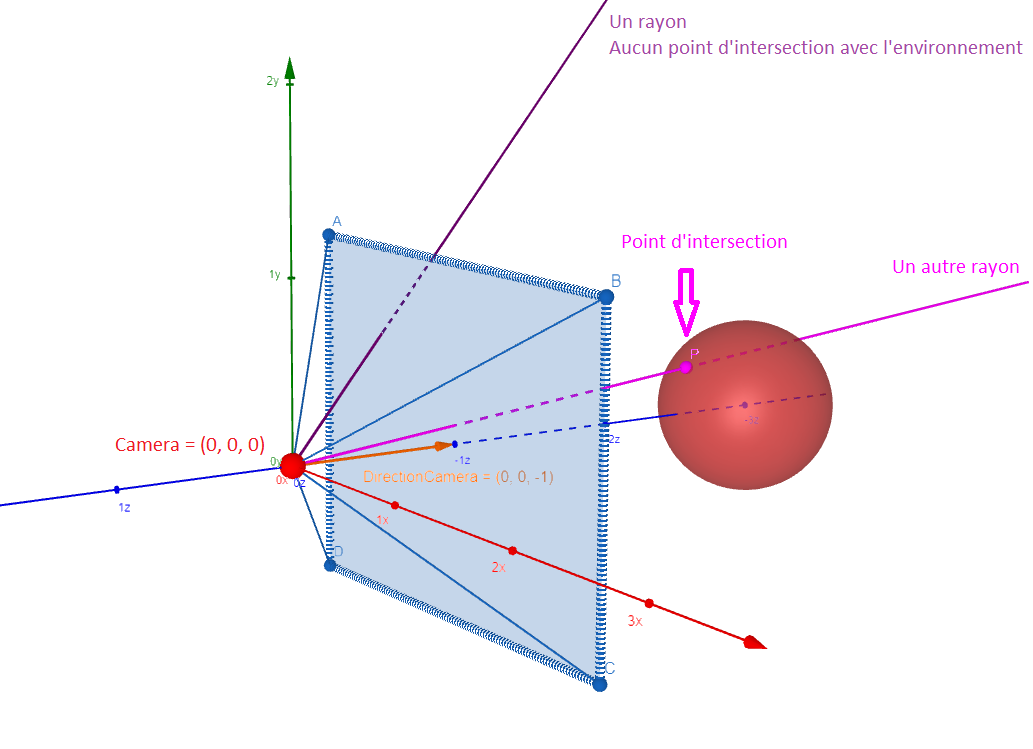
\includegraphics[width=1.1\textwidth]{img/rt/repCam2Rayonsv2.png}}

	\caption{Représentation de la caméra, de son plan, de sa direction ainsi que d'une sphère représentant l'environnement. Deux rayons sont également tracés.}
	\label{repreCamRayon}
\end{figure}
\FloatBarrier

En reprenant l'exemple de notre image de rendu en 800x600 pixels et en suivant les étapes de l'algorithme \label{conversionPixel}:\\
$P(x, y, z), x \in [0; 799], y \in [0; 599], z = -1$ :
\begin{enumerate}
	\item{\textbf{Etape 1} : On ajoute 0.5 à la valeur du pixel que l'on veut rendre. Les pixels étant des carrés de 1x1 unité sur l'image, ajouter 0.5 fera donc passer le rayon au centre du pixel. La division par la largeur et la hauteur de l'image (pour x et y respectivement) permet de ramener les coordonnées des pixels dans l'intervalle $[0; 1]$.\\
		\hfill\\
	         	$P(x, y, z), x \in [0; 1], y \in[0; 1], z = -1$}
	\item{\textbf{Etape 2} : Le but de cette étape est de ramener les pixels dans l'intervalle $[-1; 1]$.\\
		$x*2 \Rightarrow x \in [0; 2]$
		$\\x - 1 \Rightarrow x \in [-1; 1]$\\
		Même raisonnement pour y à une inversion d'opération prêt.\\
		\hfill\\
	          	$P(x, y, z), x \in [-1; 1], y \in[-1; 1], z = -1$}
	\item{\textbf{Etape 3} : Cette étape permet de prendre en compte le champ de vision de la caméra. Plus le champ de vision se rapproche de 180\degree, plus la caméra voit une grande partie de la scène et inversement. Le champ de vision peut alors donner une impression de "zoom". Voir plus bas la \figurename~\ref{fovCam}\\\hfill\\
		$P(x,y , z), x \in [-1; 1]*FOV, y \in [-1; 1]*FOV, z = -1$.}\\
	\item{\textbf{Etape 4} : Jusqu'alors, les coordonnées de nos pixels converties dans l'espace du monde formaient un plan de caméra carré. Comment faire si l'image que nous voulons rendre n'est pas elle-même carrée (ce qui est très fréquent) ? Il nous faut prendre en compte le format de l'image donné par $width/height$. En multipliant la coordonnée x par ce format, nous "étirons" l'image ou la rétrécissons selon sa largeur. Le plan de la caméra respecte maintenant le même format que l'image que nous voulons rendre.\\\hfill\\
		$P(x,y , z), x \in [-1; 1]*FOV*aspectRatio, y \in [-1; 1]*FOV, z = -1$.}
\end{enumerate}

\begin{figure}[h!]
	\adjustbox{center}{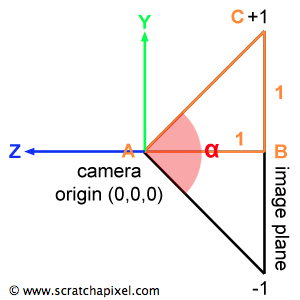
\includegraphics[width=0.5\textwidth]{img/rt/fovCamera.png}}

	\caption{En augmentant le FOV (champ de vision) de la caméra, l'angle $\alpha$ augmente. La hauteur du plan de la caméra, $BC$, est étirée. La caméra verra donc une plus grande partie de la scène. \textbf{Source: scratchapixel.com}}
	\label{fovCam}
\end{figure}
\FloatBarrier

A l'issue de ces implémentations, nous obtenons alors l'image suivante (la scène est composée d'une unique sphère rouge et d'un fond gris foncé):

\begin{figure}[h!]
	\adjustbox{center}{
\includegraphics[width=0.5\textwidth]{img/rt/basicRender.png}}

	\caption{Rendu le plus simple. Une sphère sans aucun effet d'ombrage}
	\label{basicRender}
\end{figure}
\FloatBarrier

Chaque rayon qui a été lancé et qui a intersecté la sphère a alors donné un pixel rouge. Les autres rayons, ceux qui n'ont pas intersecté la sphère, ont simplement renvoyé la couleur du fond de la scène. 

\subsubsection{L'ombrage de Phong}
\label{ombragePhong}

Comme vu précédemment, la première image (fig. \ref{basicRender}) produite par notre algorithme n'est pas tout à fait satisfaisante. Il n'y a en effet aucun effet de profondeur ou de lumière. Difficile de savoir qu'on a une sphère devant nous et non un simple disque plat. La prochaine étape est donc celle de l'ombrage de Phong. Un tel ombrage se découpe en trois composantes/parties:
\begin{enumerate}
	\item{La composante ambiante. Elle est responsable de la quantité minimale de lumière que va reçevoir un objet}
	\item{La composante diffuse. Cette composante est celle qui permet de donner à un objet son relief. Plus les rayons de la lumière arrivent perpendiculairement à la surface de l'objet, plus l'intensité lumineuse sur la surface de l'objet sera importante}
	\item{La composante spéculaire. Elle permet d'ajouter un effet "brillant" aux objets en fonction de la direction qu'empruntent les rayons réfléchis par la surface de l'objet par rapport à la caméra.}
\end{enumerate}

\hfill\\
\indent La composante ambiante permet de donner une illumination de base à l'objet. En temps normal, même si un objet n'est pas directement éclairé par la source de lumière, il est tout de même visible dans la plupart des cas. C'est parce que la lumière de la source lumineuse rebondit dans la scène et les rayons arrivent indirectement éclairer l'objet. C'est ce que l'on appelle l'illumination globale. L'illumination globale est capable de génèrer des images fortes de réalisme mais est très coûteuse en temps de calcul. La composante ambiante de l'ombrage de Phong approxime très simplement cet effet en donnat une "luminosité mininale" à toute la scène. La composante ambiante est très simple à calculer:\\

\begin{center}
	$Ambiante = I_A = S_A*I_L$
\end{center}
Avec $I_L\ \in\ [0;1]$ l'intensité de la source lumineuse,\\
$S_A\ \in\ [0; 1]$ l'intensité de la lumière ambiante dans la scène. Ce paramètre affecte donc tous les objets de la scène.

\begin{figure}[h!]
	\adjustbox{center}{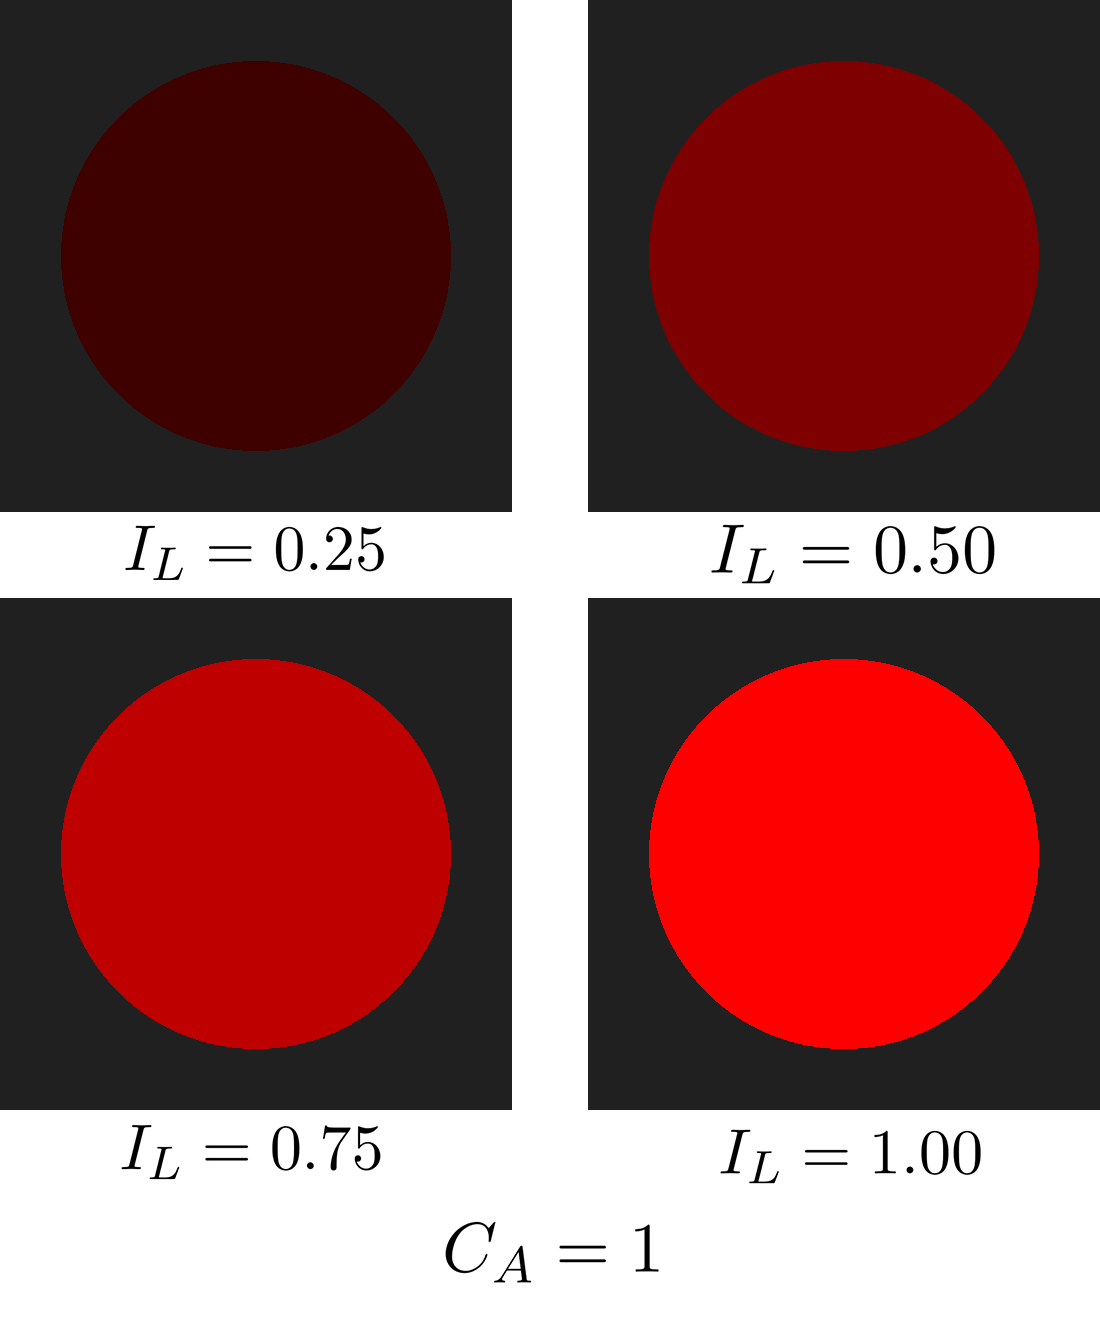
\includegraphics[width=0.5\textwidth]{img/rt/differentAmbient.png}}

	\caption{Le rendu de la même sphère pour différentes intensités lumineuse $I_L$. $C_A = 1$ utilisé pour tous les rendus.}
	\label{differentAmbient}
\end{figure}
\FloatBarrier

La composante diffuse de l'ombrage de Phong permet d'ajouter un effet que l'on peut voir comme un dégradé d'intensité lumineuse. L'intensité est à son maximum lorsque les rayons de la source lumineuse frappent perpendiculairement la surface de l'objet. Au contraire, lorsque les rayons sont parallèles à la surface de l'objet, l'intensité lumineuse de la diffusion est très faible. Elle est calculée comme suit:\\

\begin{center}
	$Diffuse = I_D = C_D*(\overrightarrow{L}\cdot\overrightarrow{N})$
\end{center}
Avec $C_D$ le coefficient d'intensité diffuse de l'objet,\\
$\overrightarrow{L}$ le vecteur en direction de la source lumineuse depuis le point d'intersection du rayon et de l'objet,\\
$\overrightarrow{N}$ la normale de la surface de l'objet au point d'intersection avec le rayon\\
et $\cdot$ dénotant le produit scalaire.\\
On sait que le produit scalaire de deux vecteurs orthogonaux est égal à 0. De plus, le produit scalaire de deux vecteurs colinéaires normalisés (de longueur 1) vaut 1. Ainisi, deux vecteurs normalisés non-colinéaires et non-orthogonaux auront un produit scalaire compris entre 0 et 1. Plus les vecteurs sont similaires, plus le produit se rapprochera de 1 et à l'inverse, "plus les vecteurs sont orthogonaux" plus il tendra vers 0.\\
Appliqué au cas de notre sphère et de notre source de lumière :\\
\begin{itemize}
	\item{Si le vecteur représentant la direction du rayon de lumière (le vecteur entre le point d'intersection sur l'objet et la source lumineuse) est colinéaire à la normale au point d'intersection de l'objet, l'intensité de la composante diffuse sera maximale car le produit scalaire des deux vecteurs vaudra alors 1.}
	\item{Si au contraire, la lumière frappe l'objet de côté, la normale et le vecteur du rayon de lumière seront alors orthogonaux (ou presque), le produit scalaire vaudra 0. L'intensité de la composante diffuse sera minimale.}
\end{itemize}


\begin{figure}[h!]
	\adjustbox{center}{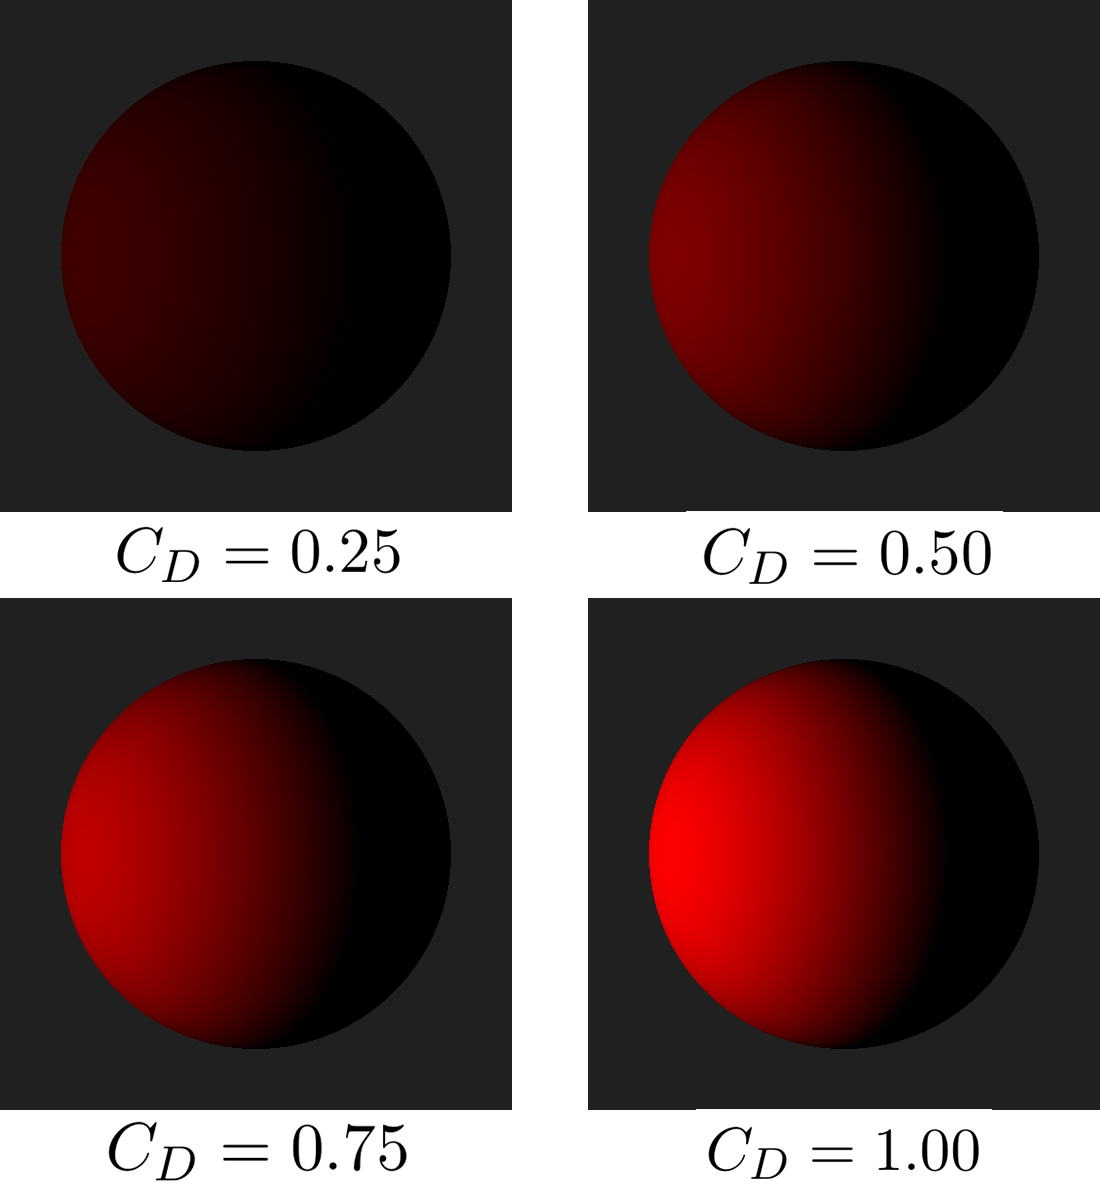
\includegraphics[width=0.5\textwidth]{img/rt/differentDiffuse.png}}

	\caption{Le rendu de la même sphère pour différents coefficients de diffusion $C_D$ de l'objet. On devine la position de la source lumineuse à gauche.}
	\label{differentDiffuse}
\end{figure}
\FloatBarrier

La dernière composante est la spéculaire. Elle est responsable des points de reflets qu'on peut voir dans la vraie vie sur des objets en plastique notamment. L'idée de son fonctionnement est la suivante:\\
Plus le rayon de lumière qui frappe l'objet en un point donné est réfléchi droit sur la caméra, plus l'intensité spéculaire en ce point est importante. Le calcul de la spécularité:

\begin{center}
	$Specularite = I_S = C_S*(\overrightarrow{d_{ray}}\cdot\overrightarrow{R_{light}})^\alpha$
\end{center}
$C_S$ étant le coefficient d'intensité spéculaire de l'objet,\\
$\overrightarrow{d_{ray}}$ la direction du rayon qui a intersecté l'objet,\\
$\overrightarrow{R_{light}}$ la direction du rayon de lumière entre la source de lumière et le point d'intersection s'il est parfaitement réfléchi (voir la partie \ref{reflexions} sur les réflexions) par rapport à la surface de l'objet,\\
$\alpha$ la "brillance" de l'objet. Plus ce paramètre est élevé plus les tâches spéculaires seront petites. L'objet paraîtra plus brillant.

D'une façon analogue au fonctionnement de la composante diffuse, plus le produit scalaire des vecteurs $\overrightarrow{R_{light}}$ et $\overrightarrow{d_{ray}}$ se rapproche de 1, plus l'intensité de la spécularité sera forte.\\
Le paramètre alpha permet quant à lui de jouer sur la taille des tâches spéculaires. En effet, on observe sur la \figurename~\ref{differentSpecular}, pour $C_S = 1$ et $\alpha = 10$, que la tâche spéculaire est moins intense sur ses bords qu'en son centre.\\
On peut grossièrement estimer que l'intensité lumineuse de la spécularité $I_S$ aux bords de la tâche spéculaire est comprise entre 0.5 et 1: $0.5 \leqslant I_S \leqslant 1$.\\
Ainsi $I_S$, décroîtra rapidement vers 0 lorsque élevée à la puissance $\alpha$. A contrario, $I_S$ se rapprochant de 1 au centre de la tâche lumineuse, la décroissance vers 0 sera plus lente, bien que tout à fait présente comme en témoigne la \figurename~\ref{differentSpecular} aux paramètres $C_S = 1$ et $\alpha = 512$.

\begin{figure}[h!]
	\adjustbox{center}{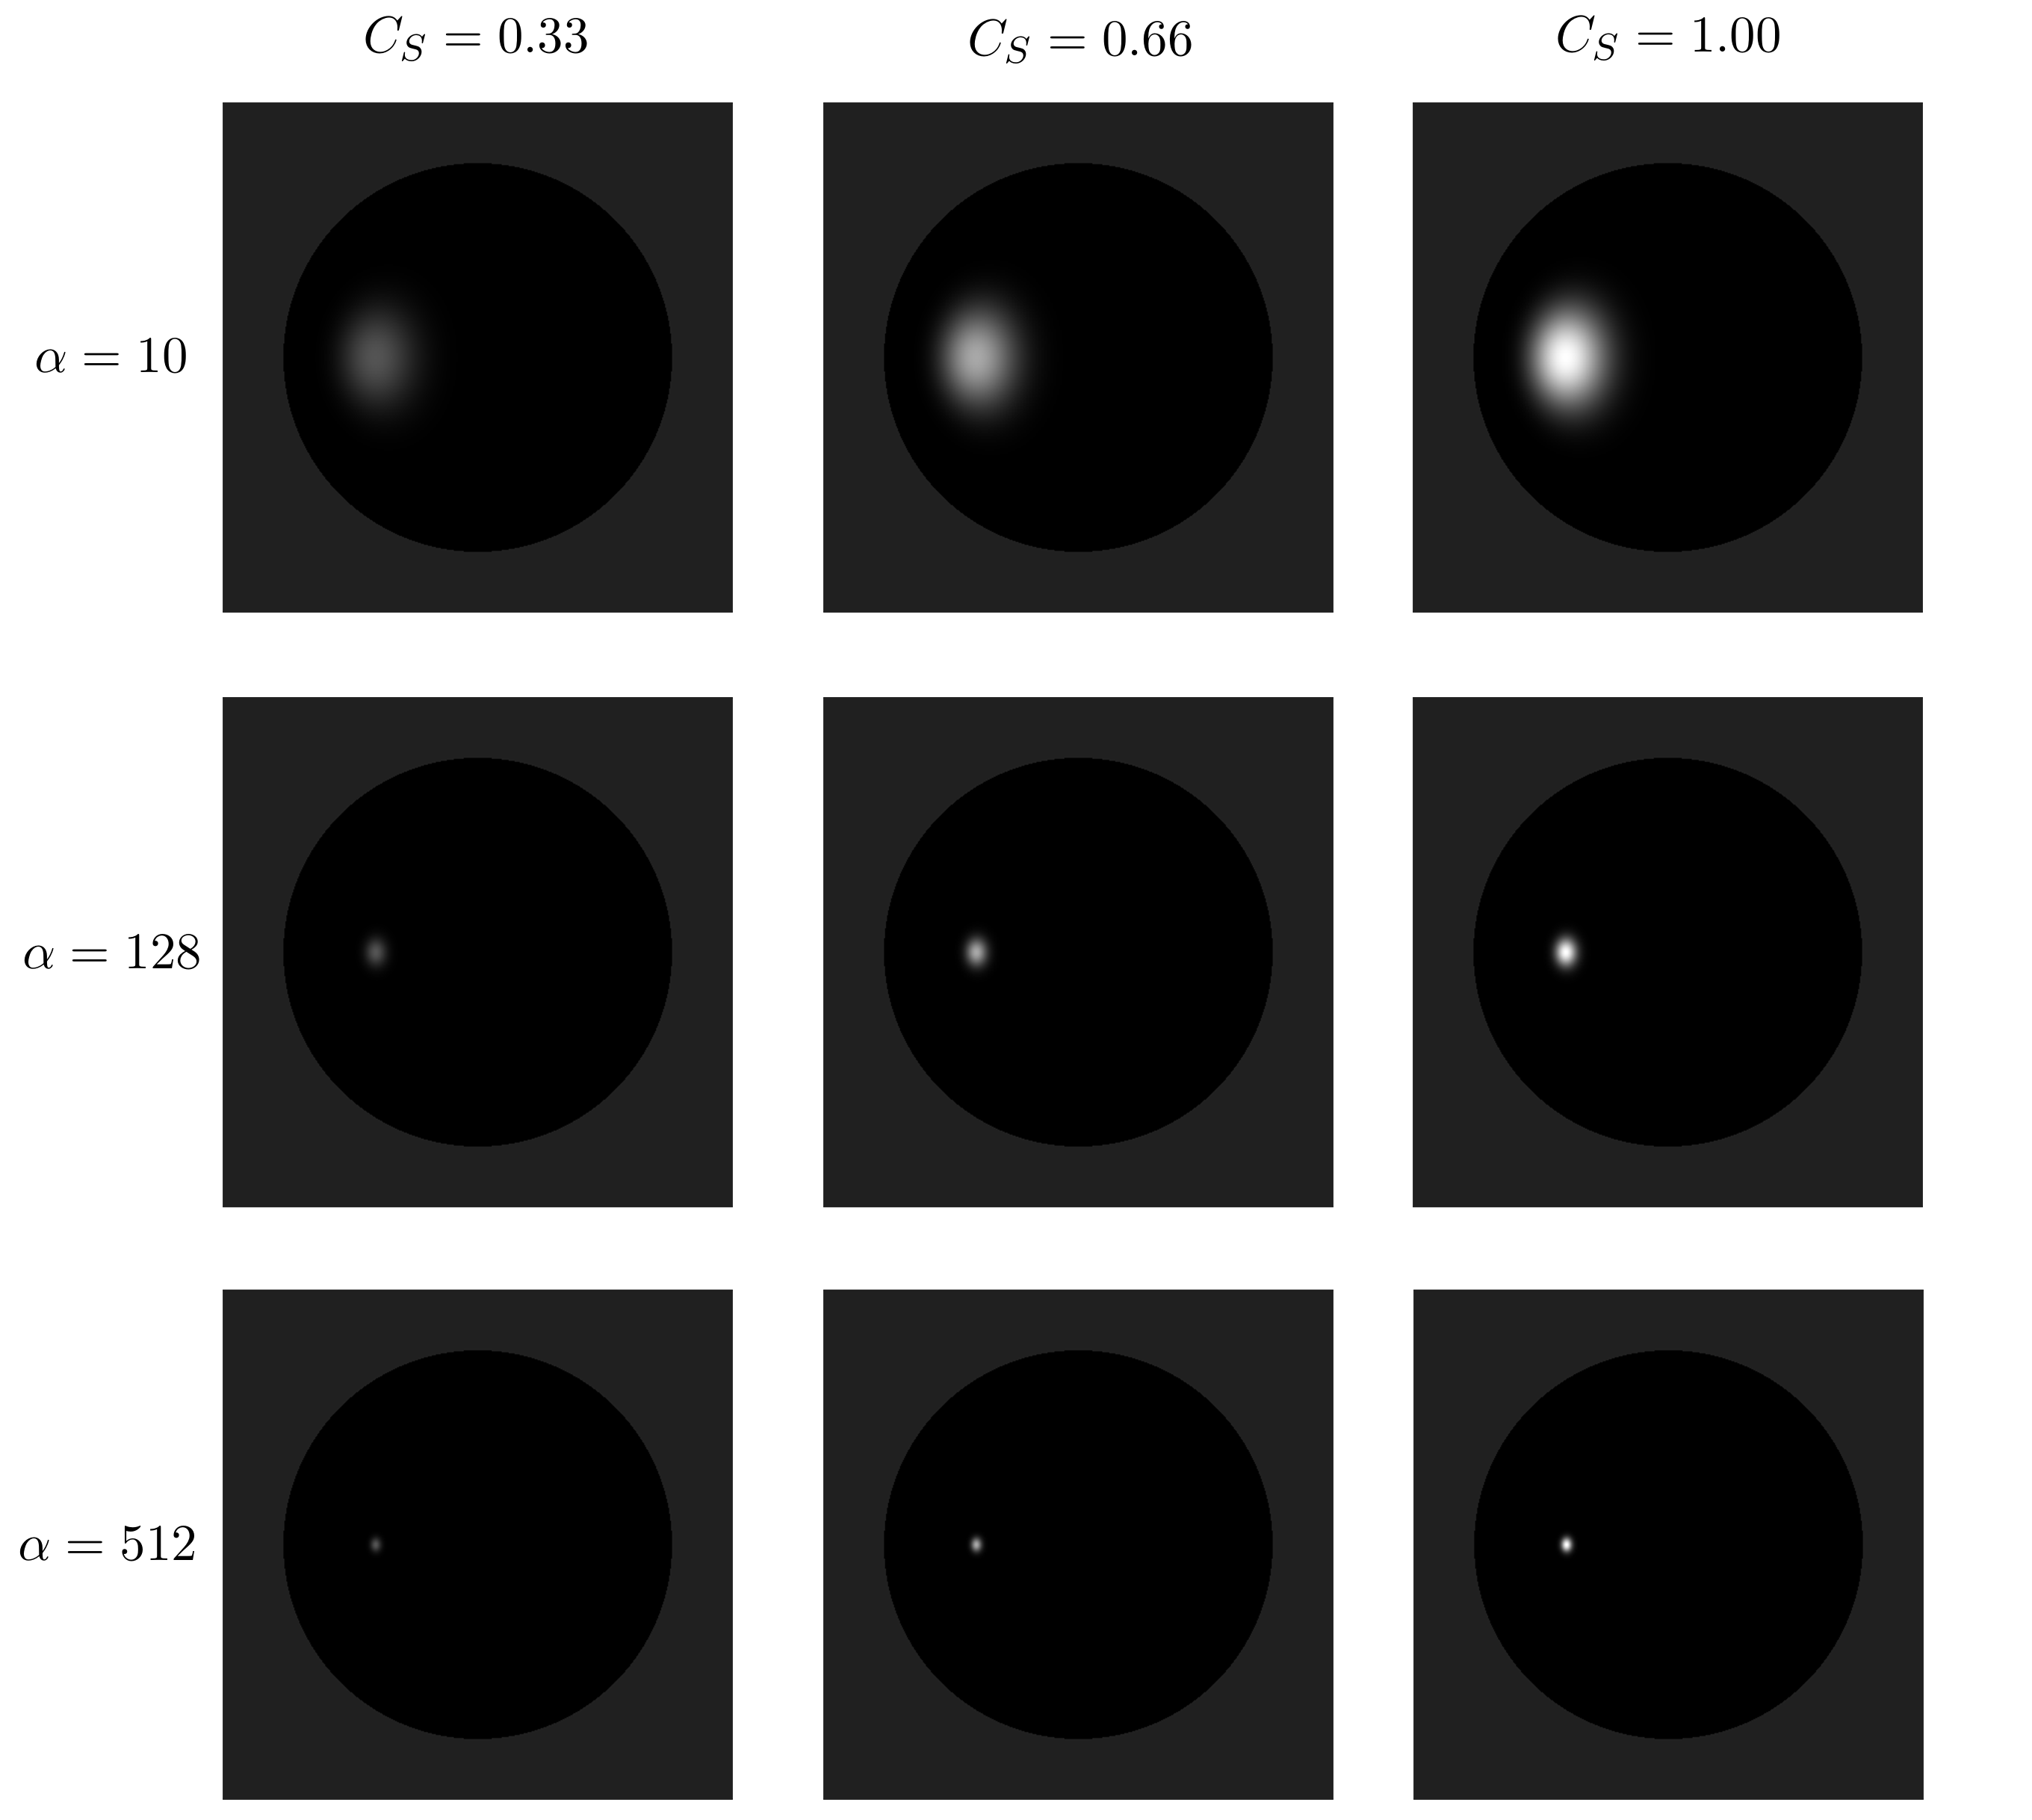
\includegraphics[width=0.8\textwidth]{img/rt/differentSpecular.png}}

	\caption{Le rendu de la même sphère pour différents coefficients de spécularité $C_S$ de l'objet et différentes valeurs du paramètre $\alpha$. La source lumineuse est à gauche.}
	\label{differentSpecular}
\end{figure}
\FloatBarrier

Les trois composantes de l'ombrage de Phong étant maintenant calculées, nous pouvons calculer l'intensité lumineuse totale en un pixel $P_{(x, y)}$ donné de l'image:
\begin{itemize}
	\item{Si le rayon passant par ce pixel n'intersecte rien, la couleur renvoyée est celle du fond de la scène}
	\item{Si le rayon intersecte un objet, la couleur renvoyée est:}
\end{itemize}
\begin{center}
$C_{P(x, y)} = C_O * IntensitePhong = C_O*(I_A + I_D + I_S)$
\end{center}
$C_O$ étant la couleur de l'objet,\\
$I_A, I_D, I_S$ sont les intensités ambiantes, diffuses et spéculaires présentées précédemment.

Pour la même sphère et la même source de lumière, nous obtenons alors:

\begin{figure}[h!]
	\adjustbox{center}{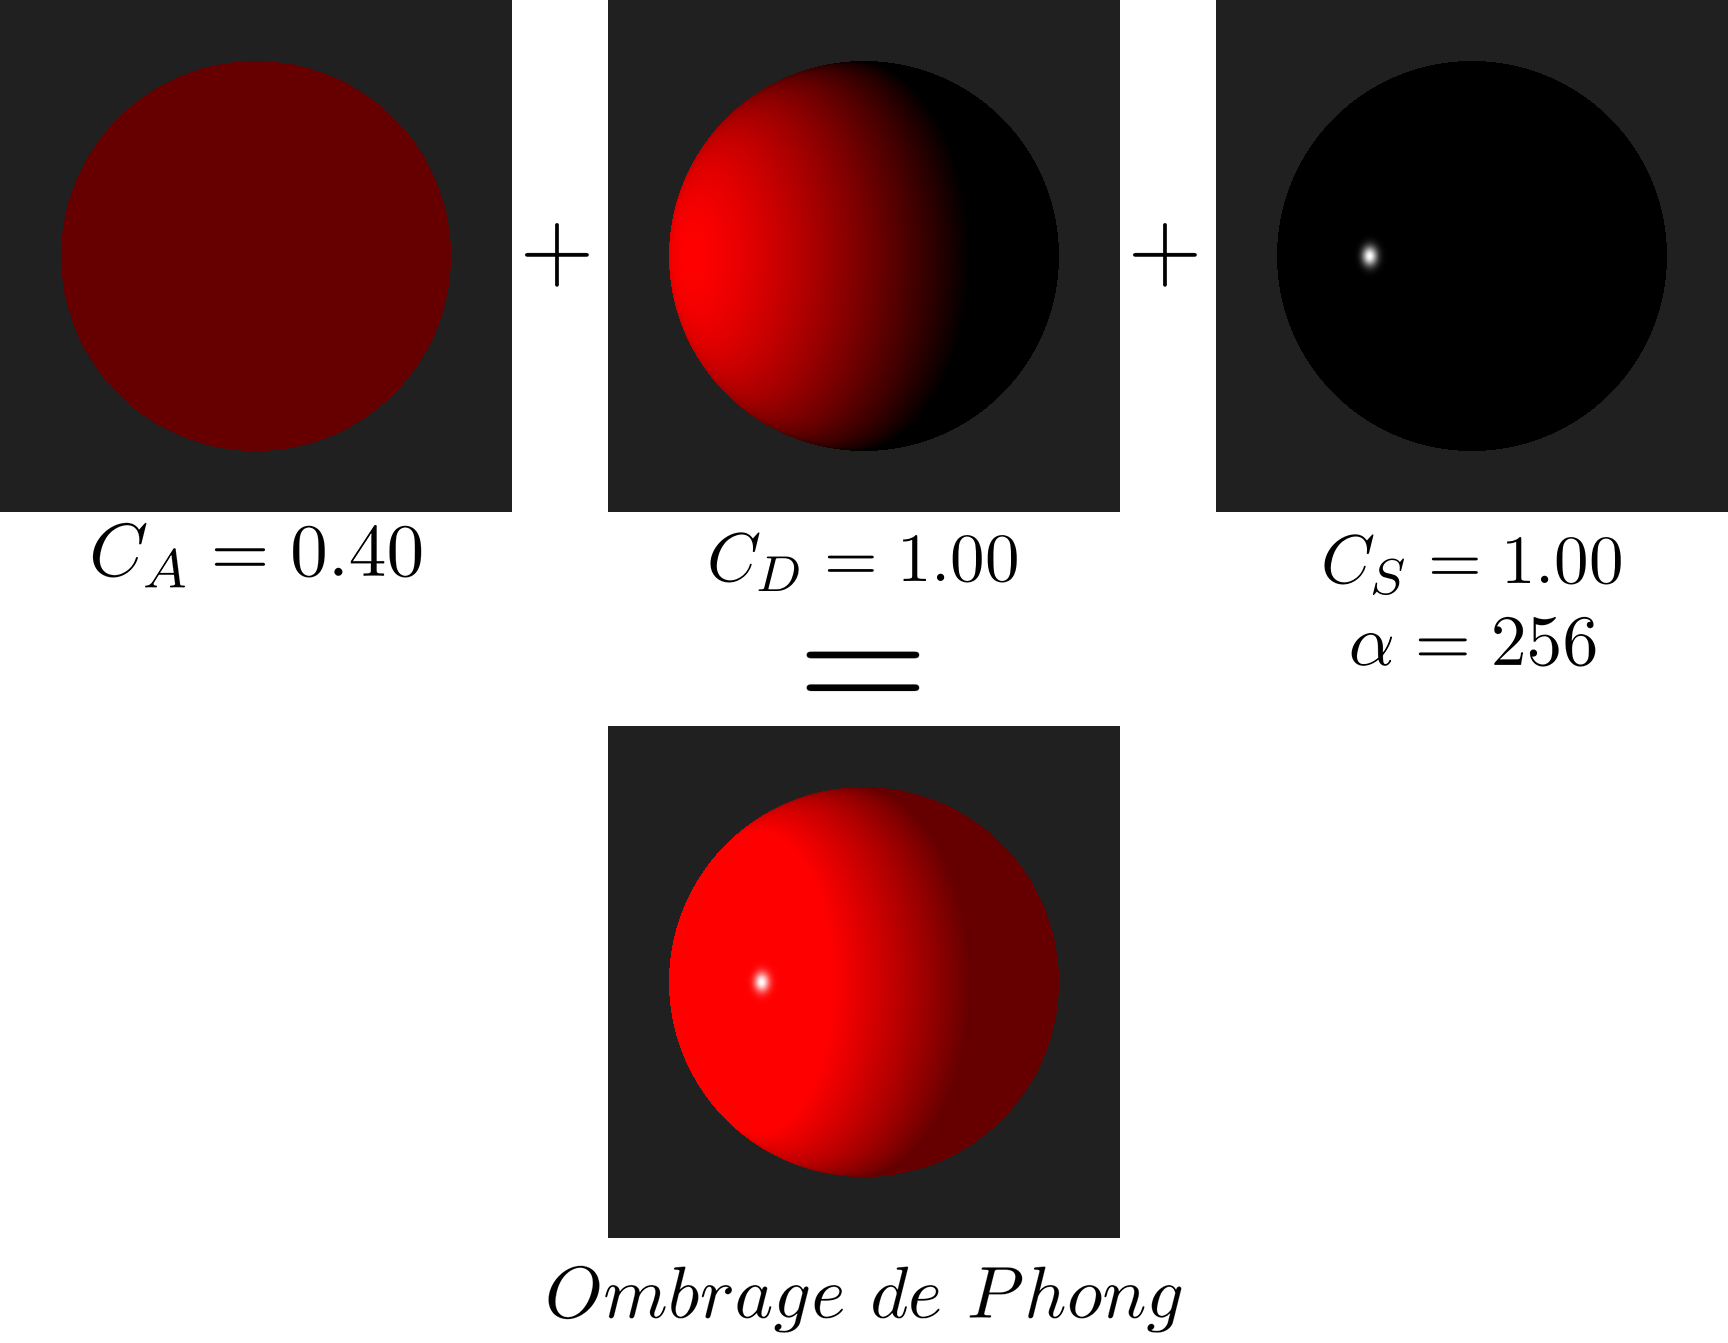
\includegraphics[width=0.75\textwidth]{img/rt/phongAddition.png}}

	\caption{Rendu final de la sphère en additionnant toutes les composantes de l'ombrage de Phong}
	\label{finalPhong}
\end{figure}
\FloatBarrier

\subsubsection{Les ombres}

Afin de rajouter un degré de réalisme au rendu, nous nous proposons de rajouter des ombres. Le principe est simple: pour chaque rayon tiré depuis la caméra, on se place au point d'intersection trouvé par le rayon avec un objet de l'environnement. Depuis ce point, on tire un autre rayon directement en direction de la source de lumière. Si ce nouveau rayon vient à intersecter quelque chose sur son chemin à la lumière, cela veut dire que nous sommes dans l'ombre. Quelque chose bloque l'accès direct à la lumière. La couleur du pixel sera alors seulement la partie ambiante de l'objet premièrement intersecté. Si ce deuxième rayon n'intersecte rien, nous ne sommes pas dans l'ombre et nous pouvons calculer l'intensité lumineuse en utilisant l'ombrage de Phong vu en partie \ref{ombragePhong}. De part leur nature, on appelle ces rayons secondaires des "shadow ray".

\begin{figure}[h!]
	\adjustbox{center}{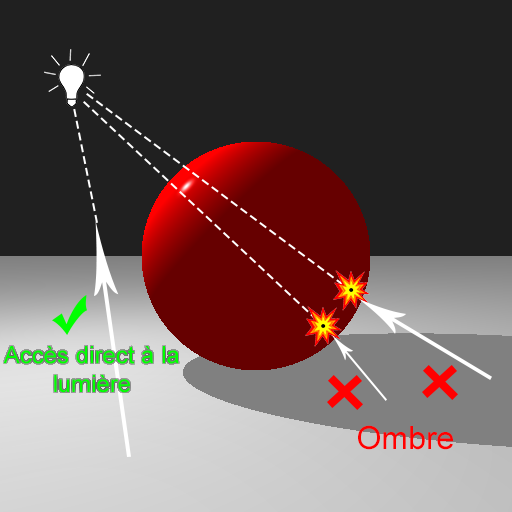
\includegraphics[width=0.5\textwidth]{img/rt/ombresSchema.png}}

	\caption{Des points d'intersection ont été trouvés avec le plan derrière la sphère. Les shadow-ray tirés depuis ces points d'intersection ne peuvent pas accéder directement à la lumière. C'est une zone d'ombre.}
	\label{ombresSchema}
\end{figure}
\FloatBarrier

L'algorithme de calcul de la couleur de chacun des pixels peut donc être adapté pour tenir compte des ces nouvelles ombres:

\begin{algorithm}[H]
	\KwIn{$x, y$ les coordonnées du pixel dont on souhaite calculer la couleur}
	\KwOut{$C_P$, la couleur du pixel\\\hfill\\}
	
	coord$_{(x, y)} \gets$ conversionPixelScene(x, y)\\
	cameraRay $\gets$ $Rayon(camera, coord_{(x, y)})$\\
	\If{cameraRay.intersects(objetScene)}
	{
		intersectedObject $\gets$ objet intersecté par $cameraRay$\\\hfill\\
		shadowRay $\gets Rayon(pointIntersection, lumiere)$\\
		\If(\tcp*[h]{Le point d'intersection est dans l'ombre}){shadowRay.intersects(objetScene)}
		{
			\Return{$Color_{intersectedObject} * I_A$}
		}
		\Else(\tcp*[h]{Nous ne sommes pas dans l'ombre})
		{
			\Return{phongShading(pointIntersection)}
		}
	}
	\Else
	{
		\Return{backgroundColor}
	}

	\caption{Algorithme retournant la couleur d'un pixel en fonction du fait qu'il soit dans l'ombre ou non - computeShadow}
	\label{algoOmbres}
\end{algorithm}

\subsubsection{Les réflexions}
\label{reflexions}

Jusqu'alors, notre algorithme n'est capable de rendre que des objets dont le matériau est matte. La spécularité peut éventuellement donner un effet de brillance mais ce n'est qu'une impression. En ajoutant des matériaux réflexifs, nous pourrons créer des objets qui réfléchissent la lumière à la façon d'un miroir ou des objets à l'aspect métallique. Le principe derrière le calcul des réflexions est le suivant:
\begin{itemize}
	\item{Si le camera-ray lancé intersecte un objet qui n'est pas réfléchissant, calculer sa couleur avec l'ombrage de Phong comme vu précédemment.}
	\item{Si le rayon intersecte un objet réfléchissant, calculer la direction du rayon réfléchi et lancer un nouveau rayon dans cette direction de façon récursive. La couleur renvoyée sera alors la dernière chose que touche le rayon (un objet non réflexif ou le fond de la scène)}
\end{itemize}
La direction d'un rayon parfaitement réfléchi peut se calculer grâce au rayon incident $I$ ainsi que grâce à la normale de la surface au point d'intersection $N$:

\begin{figure}[h!]
	\adjustbox{center}{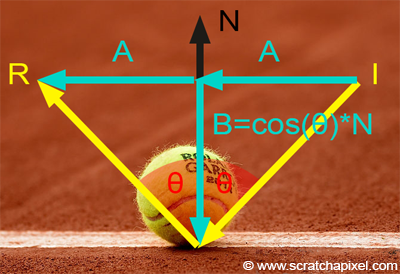
\includegraphics[width=0.5\textwidth]{img/rt/reflectionVector.png}}

	\caption{On peut calculer le rayon réfléchi à partir du rayon incident et de la normale. \textbf{Source: scratchapixel.com}}
	\label{reflectionCalcul}
\end{figure}
\FloatBarrier

La \figurename\ \ref{reflectionCalcul} nous montre qu'une balle de tennis (jouant le rôle d'un rayon) rebondira avec un angle de sortie $\theta$ égal à son angle d'arrivée ($\theta$) par rapport au sol. Le principe est le même avec les rayons. Par construction géométrique, on obtient la direction du rayon réfléchi:

\begin{center}
	$\overrightarrow{R} = \overrightarrow{I} - (\overrightarrow{N}\cdot \overrightarrow{I})*\overrightarrow{N}*2$
\end{center}

Il ne reste plus, pour calculer la couleur de la réflexion, qu'à prendre en compte le coefficient de réflexion $C_R$ du matériau. On obtient alors l'algorithme:

\begin{algorithm}[H]
	\DontPrintSemicolon
	\KwIn{$\overrightarrow{R}$ le rayon incident, $depth$ la profondeur actuelle}
	\KwOut{La couleur du pixel $P_{(x, y)}$ par lequel est passé le camera-ray initial\\\hfill\\}

	\If(\tcp*[h]{La profondeur de récursion maximale a été atteinte}){depth == 0}
	{
		\Return{backgroundColor}
	}
	\hfill\\

	\If(\tcp*[h]{On vérifie si on a intersecté quelque chose}){$\overrightarrow{R}$.intersects(objetsScene)}
	{
		intersectedObject $\gets$ objet intersecté par $\overrightarrow{R}$\\\hfill\\

		\If(\tcp*[h]{Si l'objet intersecté est réfléchissant}){intersectedObject.isReflexive()}
		{
			$\overrightarrow{R_{reflect}} \gets$ computeReflectedDirection($\overrightarrow{R}$, $\overrightarrow{N}$)\\\hfill\\

			\Return{$C_R*$computeReflection($\overrightarrow{R_{reflect}}$, depth - 1)}{\tcp*[h]{On effectue un appel récursif pour relancer un rayon}}
		}
		\Else(\tcp*[h]{L'objet n'est pas réfléchissant, on va simplement retourner son ombrage de Phong})
		{
			\Return{phongShading()}
		}
	}
	\Else
	{
		\Return{backgroundColor}
	}

	\caption{Algorithme de calcul des réflexions pour des objets non colorés - computeReflection}
	\label{algoReflections}
\end{algorithm}

Cet algorithme suppose que l'objet n'est pas coloré et donc qu'il renvoie les rayons tels quels. Dans le cas d'un objet métallique cependant, un lingot d'or par exemple, la réflexion sera colorée par la couleur du matériau. La méthode n'est pas présentée ici car il ne s'agit que de montrer le principe des réflexions.

\begin{figure}[!h]
	\adjustbox{center}{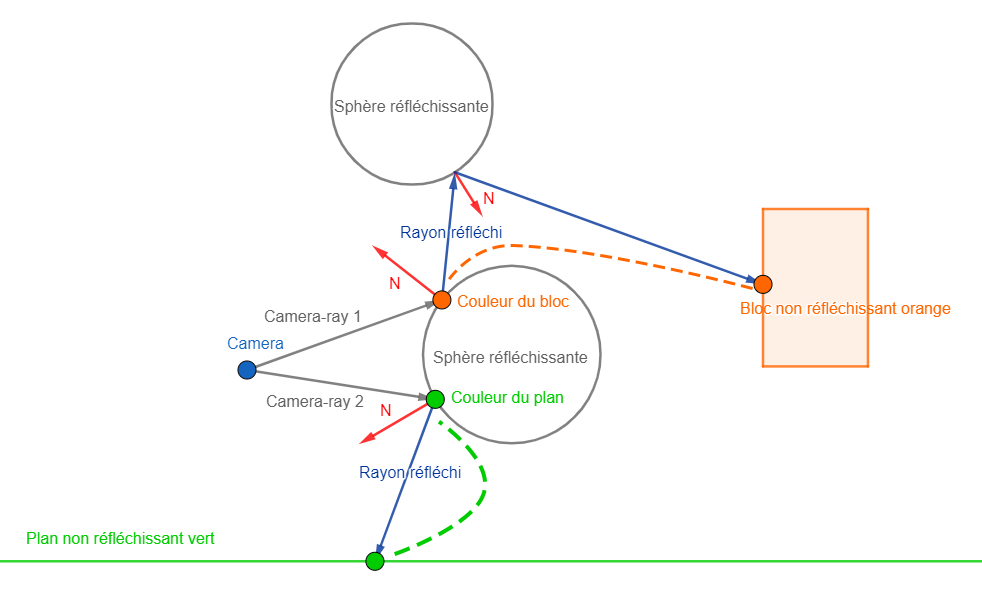
\includegraphics[width=1.1\textwidth]{img/rt/reflectionsSchema.png}}

	\caption{Exemple de rebonds successifs des rayons jusqu'à un objet non réfléchissant}
	\label{reflectionsSchema}
\end{figure}
\FloatBarrier

La \figurename\ \ref{reflectionsDemo} montre un résultat que l'ont peut obtenir avec deux sphères réflexives (une au centre et une à sa droite), plusieures sphères mattes ainsi qu'un plan:

\begin{figure}[h!]
	\adjustbox{center}{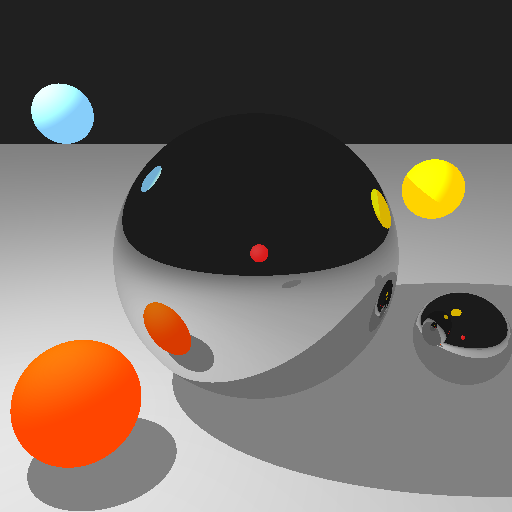
\includegraphics[width=0.5\textwidth]{img/rt/reflectionsDemo.png}}

	\caption{On peut voir une sphère rouge derrière la caméra grâce à la reflexion de la sphère centrale. Les coefficients de réflexion ont été fixés à 0.8 pour ce rendu.}
	\label{reflectionsDemo}
\end{figure}
\FloatBarrier

La prochaine étape consistera à ajouter le support des objets transparents en implémentant un système de réfraction des rayons.
\subsubsection{Les réfractions}

\subsection{Le multithreading}

Les algorithmes de Ray Tracing sont capables de générer des images réalistes mais sont, en contrepartie, assez lents à exécuter. Un avantage cependant de ces algorithmes est que chaque pixel est calculé indépendamment des autres. Il n'y a pas besoin d'attendre que le "pixel 1" soit calculé pour pouvoir calculer le pixel 2". Tous les pixels sont indépendants des autres. Cela fait donc de ces algorithmes des cibles parfaites pour la parallélisation des calculs. Dans le cas de notre implémentation, elle est executée par le processeur de l'ordinateur. Nativement, notre programme n'était pas parallélisé et seul un des processeurs du CPU de la machine s'attelait à la tâche. L'idée était alors d'utiliser toute la puissance du CPU mise à disposition pour accélérer les temps de rendu. Pour ce faire, l'image à rendre est tout d'abord découpée en tuiles:

\begin{figure}[h!]
	\adjustbox{center}{\includegraphics[width=0.5\textwidth]{img/rt/grilleMUltithreading.png}}

	\caption{L'image que l'on veut rendre est découpée en tuiles}
	\label{grilleMultithreading}
\end{figure}



Faire un diagramme de classe pour montrer comment la classe TileTask hérite de la classe Thread de java etc...

\section{Structuration du projet}
\subsection{Les packages}
\subsubsection{Liés au Ray Tracer}




\end{document}